\documentclass[a4paper]{article}

\usepackage[dutch]{babel}
\usepackage{amsmath}
\usepackage{listings}
\usepackage{graphicx}
\usepackage{a4wide}

\setlength{\parindent}{0cm}

\title{Project Software-Ontwikkeling I: \\
       Behaviour-based robotics}
\author{Pieter De Baets \\
        Jasper Van der Jeugt \\
        Groep 31}
\date{\today}

\begin{document}

\maketitle
\subsection*{Klasse structuur}
\begin{figure}
\begin{center}
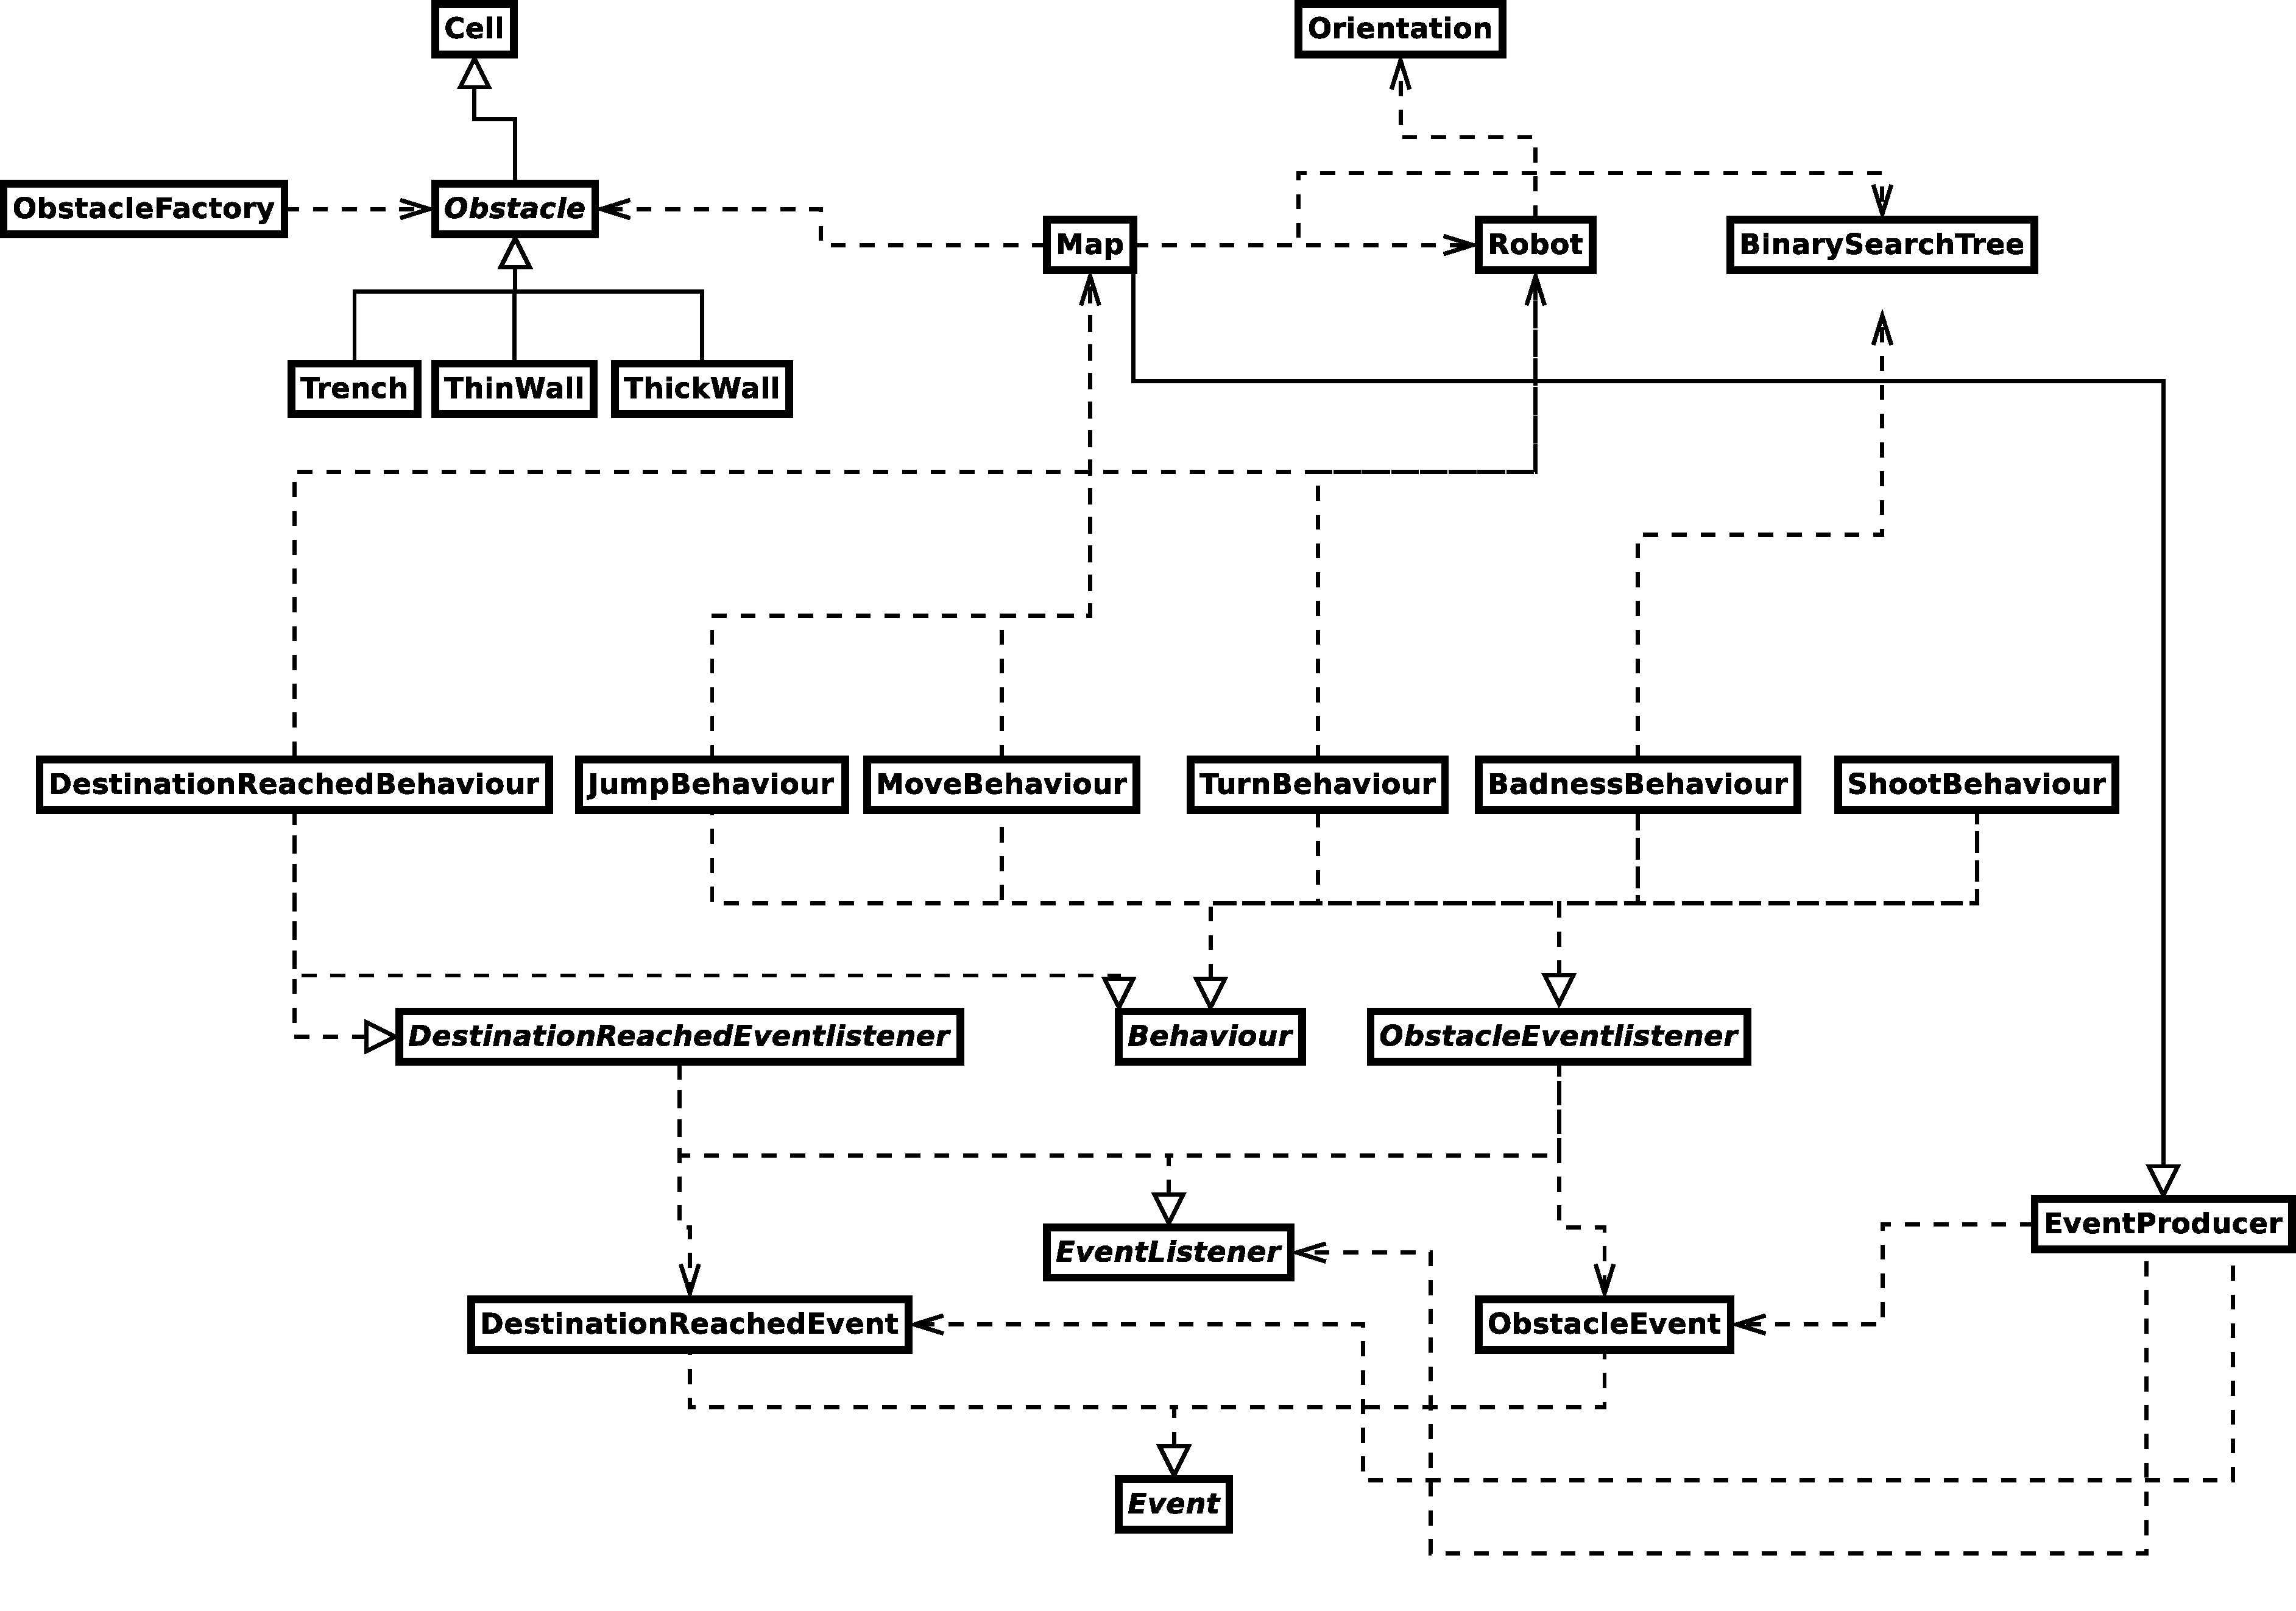
\includegraphics[width=\textwidth]{diagram.pdf}
\caption{Een diagram dat de klassestructuur van het programma toont.}
\label{fig:diagram}
\end{center}
\end{figure}

\subsection*{Ontwerpbeslissingen}
\subsubsection*{Factories voor het aanmaken van obstakels}
We besloten het Factory-design pattern te gebruiken om obstakels aan te maken.
Dit leek ons een elegante keuze, omdat we zo op een eenvoudige manier een
\verb#string# kunnen linken aan een \verb#Obstacle#. Voor elk type van
\verb#Obstacle# (\verb#Trench#, \verb#ThinWall# en \verb#ThickWall#) moet er
dus ook een \verb#ObstacleFactory# bestaan. Omdat dit tot veel herhaling zou
leiden qua code, gebruikten we templates, zodat we deze drie klassen konden
implementeren in \'e\'en algemene klasse, namelijk \verb#TObstacleFactory#.

\subsubsection*{EventProducer}
Omdat het aantal lijnen code in \verb#Map.cpp# zeer snel steeg, leek het ons een
goed idee deze klasse verder op te spitsen. We splitsten het deel dat op een
abstracte manier met events omgaat af in een klasse \verb#EventProducer#. Op
deze manier wordt de code van \verb#Map# iets overzichtelijker.

\subsubsection*{BinarySearchTree}
Volgens het principe van \emph{information hiding} beslisten we van
\verb#TreeElement# een \verb#private# \verb#nested# klasse te maken. Ook leek
het ons interessant om een balanceringsmechanisme te implementeren. Specifiek
kozen we voor de \emph{semi-splay} techniek.

\subsubsection*{BadnessBehaviour}
Om de meer geavanceerde maps op te lossen implementeerden we een extra
\verb#Behaviour# klasse. Deze klasse werkt door een bepaalde score
(\verb#badness#) te geven aan reeds bezochte plaatsen. Door dit systeem zal
de robot de gehele map proberen te verkennen.

\subsection{Wie deed wat?}

\end{document}
